% Copyright 2026 Sreeram Anil
% SPDX-License-Identifier: CC-BY-4.0
% =============================================================================
%  Second-order divided-difference filter (DD2 / CDKF) — classical Kalman family
% =============================================================================
\chapter{Second-Order Divided-Difference Filter (CDKF/DD2)}
\label{ch:cdkf}

\section*{At a glance}
\begin{tabular}{@{}l>{\raggedright\arraybackslash}p{0.76\textwidth}@{}}
Family & classical Kalman (sigma-point) \\
Header & \texttt{include/estkit/filters/cdkf.hpp} \\
Registered name & \texttt{CDKF} \\
State dimension & $n_x = 4$ (cell model) --- generic in $n_x, n_u, n_y$ \\
Evaluation points & $2n_x+1 = 9$ per stage; interpolation step $h=\sqrt3$ \\
Cost per step & $\mathcal{O}(n_x^3)$ plus $2(2n_x{+}1)$ model calls; $1.28$--$1.39\,\SI{}{\micro\second}$/step \\
Primary references & \cite{norgaard2000,ito2000gaussian,schei1997,vandermerwe2001srukf} \\
\end{tabular}

\section{Motivation and aerospace/BMS relevance}
Nørgaard, Poulsen and Ravn~\cite{norgaard2000} arrived at a sigma-point filter from a
completely different direction than Julier and Uhlmann: rather than matching moments of a
distribution, replace the Taylor expansion of $f$ and $h$ by \emph{Stirling's interpolation
formula}, which is the polynomial interpolation analogue of a Taylor series with derivatives
replaced by central divided differences. The resulting DD1 (first-order) and DD2
(second-order) filters need no derivatives, have one scalar parameter with a clean
interpretation (the interpolation step $h$), and --- in the DD2 case --- carry an explicit
second-difference term that the EKF, the UKF and the third-degree CKF all lack.

For a battery model this term is exactly the OCV curvature. Karlgaard and
Schaub~\cite{karlgaard2007huber} used the divided-difference filter as the base for robust
entry-navigation filters at NASA Langley for the same reason: it is the cheapest way to get a
second-order-accurate covariance without analytic Hessians. van der Merwe and
Wan~\cite{vandermerwe2001srukf} later showed that the DD2 filter is a member of the
sigma-point family and renamed it the central-difference Kalman filter (CDKF); the two names
refer to the same algorithm and this chapter uses them interchangeably.

\section{Problem statement and assumptions}
Model \eqref{eq:ekf-proc}--\eqref{eq:ekf-meas} with additive noise. No differentiability is
required, but the interpolation is only meaningful if $f$ and $h$ are continuous over the
stencil, i.e. over $\pm h\sigma$ along every principal axis of $\mP$. The filtering density
is again assumed Gaussian.

\begin{remark}[Notation]
Following the primary reference, $h$ without arguments denotes the scalar interpolation step
length, while $h(\cdot,\cdot)$ with two arguments is the measurement function of
\eqref{eq:ekf-meas}. The two never appear in the same role.
\end{remark}

\section{Derivation}
\paragraph{Stirling interpolation.} For a scalar function $\phi$ of a scalar argument, the
second-order Stirling formula about $\bar{s}$ with step $h$ is
\begin{equation}
\phi(\bar{s}+\delta) \approx \phi(\bar{s}) + \frac{\delta}{h}\,\tilde\mu\delta\phi(\bar s)
 + \frac{\delta^2}{2h^2}\,\delta^2\phi(\bar s),
\label{eq:cdkf-stirling}
\end{equation}
where $\tilde\mu\delta\phi(\bar s) = \tfrac12[\phi(\bar s{+}h)-\phi(\bar s{-}h)]$ is the mean
central difference and $\delta^2\phi(\bar s) = \phi(\bar s{+}h)-2\phi(\bar s)+\phi(\bar s{-}h)$
is the second central difference. This is a Taylor series with $\phi'$, $\phi''$ replaced by
their finite-difference estimates.

\paragraph{Multivariate form.} Let $\mP = \mS_x\mS_x^\T$ and write $\vx = \bar\vx + \mS_x\vz$
with $\vz \sim \N{\bm0}{\mI}$, so that the transformed coordinates are decorrelated.
Applying \eqref{eq:cdkf-stirling} coordinatewise to $g(\bar\vx + \mS_x\vz)$ and taking
expectations over $\vz$ gives (\cite[Eqs.~(30)--(34)]{norgaard2000})
\begin{align}
\E{g} &\approx \frac{h^2-n_x}{h^2}\,g(\bar\vx)
 + \frac{1}{2h^2}\sum_{i=1}^{n_x}\left[g_i^+ + g_i^-\right],
\label{eq:cdkf-mean}\\
\operatorname{Cov}\left[g\right] &\approx \mD^{(1)}\mD^{(1)\T} + \mD^{(2)}\mD^{(2)\T},
\label{eq:cdkf-cov}\\
\operatorname{Cov}\left[\vx,g\right] &\approx \mS_x \mD^{(1)\T},
\label{eq:cdkf-cross}
\end{align}
where $g_i^\pm = g(\bar\vx \pm h\,\bm{s}_i)$ with $\bm{s}_i$ the $i$-th column of $\mS_x$, and
the two divided-difference matrices have columns
\begin{equation}
\mD^{(1)}_{:,i} = \frac{g_i^+-g_i^-}{2h}, \qquad
\mD^{(2)}_{:,i} = \frac{\sqrt{h^2-1}}{2h^2}\left(g_i^+ + g_i^- - 2g(\bar\vx)\right).
\label{eq:cdkf-D}
\end{equation}
$\mD^{(1)}$ is the finite-difference stand-in for the Jacobian scaled by $\mS_x$, so
$\mD^{(1)}\mD^{(1)\T}$ is the EKF covariance term; $\mD^{(2)}$ is the genuinely new
second-order contribution, and because it enters as an outer product it can only
\emph{increase} the predicted covariance. That is the correct qualitative behaviour: the
curvature of $g$ turns a Gaussian into a skewed distribution with a larger spread.

\paragraph{Choice of $h$.} The factor $\sqrt{h^2-1}$ in \eqref{eq:cdkf-D} is what makes the
rule match the fourth moment of a Gaussian: with $h^2 = 3$ the mean weight
$(h^2-n_x)/h^2$ and the pair weight $1/(2h^2)$ coincide with the $3$-point Gauss--Hermite
weights $\{2/3, 1/6, 1/6\}$ applied at nodes $\{0,\pm\sqrt3\}$, so the DD2 filter integrates
polynomials of degree $\le 5$ exactly per axis. $h = \sqrt3$ is the value recommended in the
primary reference for Gaussian priors and the default here. Relation to the UKF: identifying
$h^2 \leftrightarrow n_x+\lambda$ makes \eqref{eq:cdkf-mean} identical to the unscented mean,
so the CDKF is a UKF with $\alpha^2(n_x+\kappa)=3$ plus the extra $\mD^{(2)}$ covariance
term.

\paragraph{Filter recursion.} Applying \eqref{eq:cdkf-mean}--\eqref{eq:cdkf-cross} to $f$ for
the time update and to $h$ for the measurement update, with $\mQ$ and $\mR$ added afterwards,
gives the algorithm below. Writing the weights explicitly,
\begin{equation}
c_1 = \frac{1}{4h^2}, \qquad c_2 = \frac{h^2-1}{4h^4}, \qquad
\operatorname{Cov}\left[g\right] = \sum_{i}\Big[c_1\,\bm{d}^{(1)}_i\bm{d}^{(1)\T}_i + c_2\,\bm{d}^{(2)}_i\bm{d}^{(2)\T}_i\Big],
\label{eq:cdkf-weights}
\end{equation}
with $\bm{d}^{(1)}_i = g_i^+-g_i^-$ and $\bm{d}^{(2)}_i = g_i^++g_i^--2g(\bar\vx)$. At
$h^2=3$: $c_1 = 1/12$, $c_2 = 1/18$.

\section{Algorithm}
\begin{algorithm}[H]
\caption{CDKF/DD2 --- one sampling period (additive noise)}
\begin{algorithmic}[1]
\Require $\xplus_{k-1},\Pplus_{k-1},\vu_{k-1},\vy_k,\vu_k$, step $h$ (default $\sqrt3$)
\State $\mS\gets\operatorname{chol}(\Pplus_{k-1})$;\;
       $f_0\gets f(\xplus_{k-1},\vu_{k-1})$;\;
       $f_i^{\pm}\gets f(\xplus_{k-1}\pm h\,\mS_{:,i},\vu_{k-1})$
\State $\xminus_k\gets\frac{h^2-n_x}{h^2}f_0+\frac{1}{2h^2}\sum_i(f_i^++f_i^-)$
\State $\Pminus_k\gets\sum_i\left[c_1(f_i^+{-}f_i^-)(\cdot)^\T+c_2(f_i^+{+}f_i^-{-}2f_0)(\cdot)^\T\right]+\mQ$
\State $\mS\gets\operatorname{chol}(\Pminus_k)$;\;
       $z_0\gets h(\xminus_k,\vu_k)$;\; $z_i^\pm\gets h(\xminus_k\pm h\,\mS_{:,i},\vu_k)$
\State $\yhat_k\gets\frac{h^2-n_x}{h^2}z_0+\frac{1}{2h^2}\sum_i(z_i^++z_i^-)$
\State $\mP_{yy}\gets\sum_i\left[c_1(z_i^+{-}z_i^-)(\cdot)^\T+c_2(z_i^+{+}z_i^-{-}2z_0)(\cdot)^\T\right]+\mR$
\State $\mP_{xy}\gets\frac{1}{2h}\sum_i \mS_{:,i}\,(z_i^+-z_i^-)^\T$
\State $\mK\gets\mP_{xy}\mP_{yy}\inv$;\; $\xplus_k\gets\xminus_k+\mK(\vy_k-\yhat_k)$;\;
       $\Pplus_k\gets\Pminus_k-\mK\mP_{yy}\mK^\T$
\State \textbf{if} constraints enabled \textbf{then} $\xplus_k\gets\Pi(\xplus_k)$
\Ensure $\xplus_k,\Pplus_k$
\end{algorithmic}
\end{algorithm}

\section{Application to the battery model}
The cell dynamics are affine in $\vx$, so every second difference $\bm{d}^{(2)}_i$ of $f$
vanishes identically and the DD2 time update collapses to the EKF time update. All of the
second-order content is in the measurement update, where
$\bm{d}^{(2)} = \ocv(\soc{+}h\sigma) + \ocv(\soc{-}h\sigma) - 2\ocv(\soc)$ is a direct
finite-difference estimate of $\ocv''\,h^2\sigma^2$. With $h=\sqrt3$ the stencil half-width is
$\sqrt3\,\sigma_\soc$, which at the initial $\sigma_\soc = 0.1$ is $0.17$ SOC --- some $35$
segments of the $241$-point OCV table, so the second difference is a smooth, well-conditioned
estimate of the curvature. In steady state ($\sigma_\soc\approx10^{-3}$) the stencil shrinks
to $\pm 0.0017$, below the table spacing $0.005$, and the second difference correctly returns
zero: the filter degenerates gracefully to the EKF when the prior is tight. This
self-scaling property is the practical advantage of a divided-difference filter over an
explicit numerical Hessian with a fixed step (Chapter~\ref{ch:soekf}).

Options: \code{h\_step = 0} (meaning $\sqrt3$), \code{second\_order = true},
\code{apply\_constraints = true}, \code{q\_scale = r\_scale = 1}.

\section{Implementation notes}
$2n_x+1 = 9$ evaluations of $f$ and $9$ of $h$ per step, plus two Cholesky factorisations;
the measured $1.28$--$1.39\,\SI{}{\micro\second}$ per step is within $5\,\%$ of the UKF, which
does the same amount of model work. Setting \code{second\_order = false} yields the DD1
filter, which is the first-order divided-difference filter (an EKF with finite-difference
Jacobians) --- useful for isolating the contribution of the $\mD^{(2)}$ term. No heap, no
recursion; \code{sizeof(Cdkf<EcmModel>)} is 4312\,bytes, the smallest of the sigma-point
filters because the evaluation points are stack temporaries rather than members. The
single-precision build reproduces the double-precision metrics to four decimals.

\section{Benchmark results}
% Copyright 2026 Sreeram Anil
% SPDX-License-Identifier: CC-BY-4.0
\begin{table}[H]\centering\footnotesize\setlength{\tabcolsep}{4pt}
\caption{CDKF: cell-level benchmark on the eVTOL mission (mean over seeds; RMSE and max error in \% SOC; $t_\mathrm{conv}$: first time the error stays below 2\,\% for 60\,s, -- = never; EKF reference: steady-state RMSE of the plain EKF on the same data).}\label{tab:cell_CDKF}
\begin{tabular}{llrrrrrcrr}\toprule
plant & scenario & RMSE & RMSE$_\mathrm{ss}$ & max & $t_\mathrm{conv}$ [s] & RMSE$_v$ [mV] & div. & EKF ref. & ns/step \\ \midrule
ECM & nominal & 0.08 & 0.05 & 1.70 & 0 & 0.81 & no & 0.05 & 1375 \\
ECM & init\_error & 1.85 & 0.12 & 7.33 & 229 & 2.11 & no & 0.05 & 1383 \\
ECM & current\_bias & 0.48 & 0.55 & 1.47 & 0 & 0.87 & no & 0.61 & 1374 \\
ECM & noise\_step & 0.14 & 0.14 & 1.70 & 0 & 2.89 & no & 0.12 & 1372 \\
ECM & outliers & 0.31 & 0.08 & 4.66 & 0 & 2.10 & no & 0.21 & 1372 \\
ECM & cold & 0.16 & 0.09 & 1.58 & 0 & 1.90 & no & 0.16 & 1372 \\
ECM & hot & 0.08 & 0.04 & 1.73 & 0 & 0.57 & no & 0.03 & 1373 \\
ECM & aged\_cell & 2.50 & 1.54 & 8.47 & 0 & 3.80 & no & 1.52 & 1372 \\
ECM & param\_mismatch & 1.84 & 1.79 & 5.19 & 0 & 2.83 & no & 1.36 & 1393 \\
ECM & sensor\_dropout & 2.75 & 1.86 & 7.45 & 0 & 1.86 & no & 0.46 & 1369 \\
ECM & preisach & 1.27 & 0.24 & 4.36 & 217 & 0.86 & no & 0.20 & 1372 \\
ECM & combined & 14.64 & 11.96 & 24.59 & -- & 5.12 & no & 12.44 & 1392 \\
\midrule
SPM & nominal & 4.70 & 4.61 & 6.13 & 0 & 1.04 & no & 3.73 & 1311 \\
SPM & init\_error & 5.26 & 4.68 & 7.33 & -- & 2.17 & no & 3.81 & 1291 \\
SPM & current\_bias & 6.05 & 6.63 & 7.46 & 0 & 1.13 & no & 5.69 & 1300 \\
SPM & noise\_step & 4.25 & 3.76 & 6.13 & 0 & 3.15 & no & 3.30 & 1311 \\
SPM & outliers & 2.26 & 2.27 & 5.67 & -- & 2.33 & no & 1.99 & 1296 \\
SPM & cold & 8.66 & 8.74 & 10.80 & -- & 4.23 & no & 7.35 & 1279 \\
SPM & hot & 2.71 & 2.71 & 3.36 & 0 & 0.72 & no & 2.16 & 1295 \\
SPM & param\_mismatch & 4.66 & 4.90 & 5.73 & 0 & 1.98 & no & 3.13 & 1304 \\
SPM & sensor\_dropout & 8.11 & 8.24 & 9.74 & 0 & 1.93 & no & 5.31 & 1296 \\
\bottomrule\end{tabular}\end{table}

\begin{figure}[H]\centering
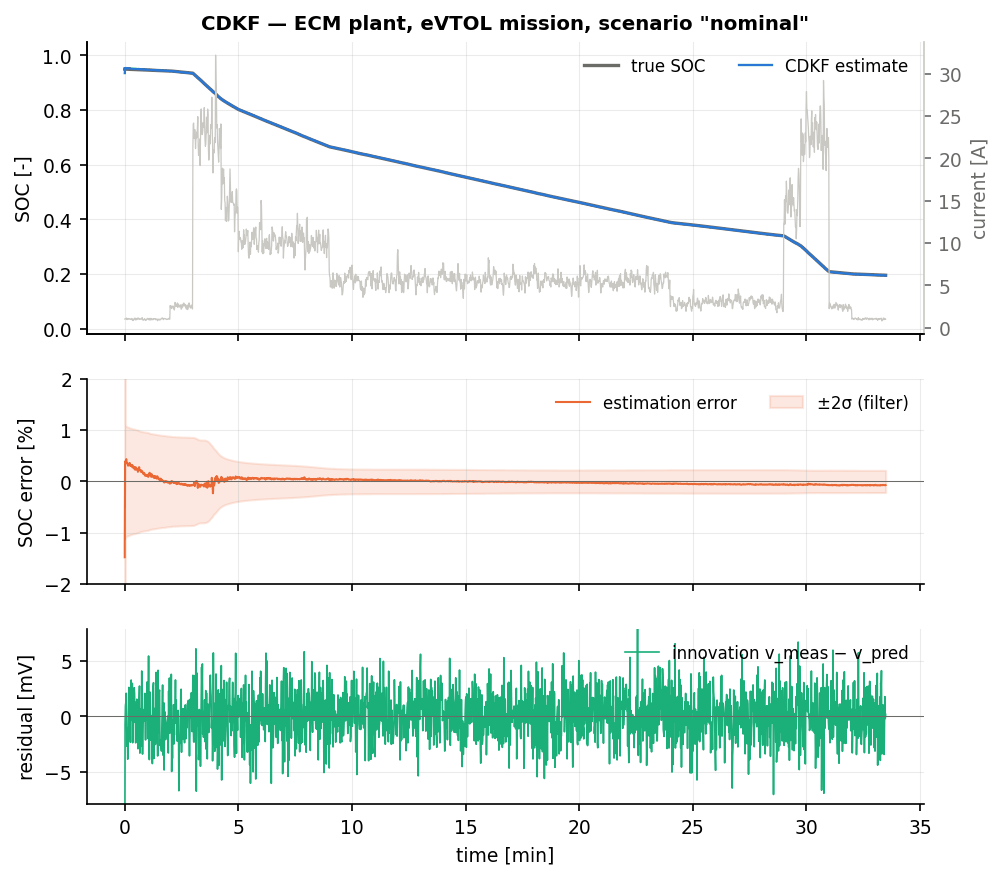
\includegraphics[width=\textwidth]{figures/cell_CDKF_nominal.png}
\caption{CDKF on the nominal eVTOL mission: true and estimated SOC (top), estimation error with the $\pm 2\sigma$ band when available (middle), voltage residual (bottom).}
\end{figure}
\begin{figure}[H]\centering
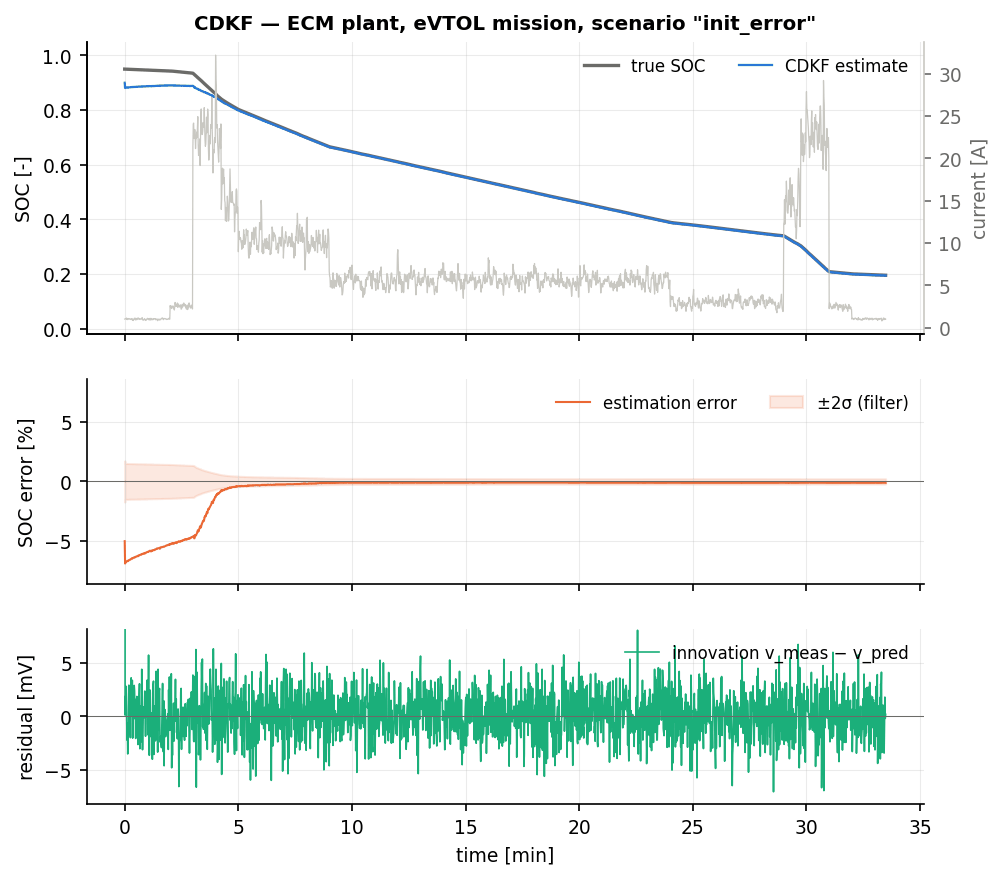
\includegraphics[width=\textwidth]{figures/cell_CDKF_init_error.png}
\caption{CDKF with a 35\,\% initial SOC error.}
\end{figure}

All numbers are three-seed means in per cent SOC.

The CDKF reproduces the fifth-degree cubature filter (Chapter~\ref{ch:ckf5}) and the $3$-point
Gauss--Hermite filter (Chapter~\ref{ch:ghkf}) to two decimals on all twelve ECM scenarios and
all nine SPM scenarios, which is the expected consequence of the three rules sharing the same
degree of exactness and, at $h^2 = 3$, essentially the same nodes. It does so with $9$ model
evaluations per stage instead of $33$ or $81$, and is therefore the \textbf{cheapest way to
obtain fifth-degree accuracy on this problem}: $1.28$--$1.39\,\SI{}{\micro\second}$ per step
against $3.7$--$4.1$ for the CKF5 and $11.2$--$12.1$ for the GHKF. That is the single most
useful practical finding of this group of chapters.

Numerically: \texttt{nominal} $0.08/0.05\,\%$ --- the equal-best whole-run RMSE of the family,
with the CKF and the two other fifth-degree rules, and better than the EKF's $0.15/0.05\,\%$
and the UKF's $0.20/0.04\,\%$; \texttt{outliers} $0.31/0.08\,\%$ with immediate convergence;
\texttt{aged\_cell} $2.50/1.54\,\%$ against the third-degree CKF's $2.87/1.79\,\%$;
\texttt{cold} $0.16/0.09\,\%$ and \texttt{hot} $0.08/0.04\,\%$, both better than the EKF's;
\texttt{current\_bias} $0.48/0.55\,\%$ against the EKF's $0.54/0.61\,\%$.

The weaknesses are those of every wide-stencil rule. \texttt{init\_error} takes $229$\,s to
converge with a whole-run RMSE of $1.85\,\%$ (steady state $0.12\,\%$), because with
$\sigma_\soc = 0.1$ the stencil reaches $\pm0.17$ SOC and the interpolating polynomial is a
poor model of the OCV over that range --- the same chord effect analysed in
Chapter~\ref{ch:ckf}. \texttt{sensor\_dropout} ($2.75/1.86\,\%$ against the EKF's
$0.72/0.46\,\%$) and \texttt{preisach} ($t_{\text{conv}} = 217$\,s against the EKF's $16$\,s)
are the same weakness seen through a fault and a bias. \texttt{param\_mismatch}
($1.84/1.79\,\%$) and \texttt{combined} ($14.64/11.96\,\%$, never converges) are model-error
scenarios where the extra integration accuracy is applied to the wrong model and does not help;
on \texttt{combined} the CDKF fails exactly as the EKF and CKF do, and for the same reason
(collapse of $\Pplus$ after the first update followed by an unmodelled $25\,\%$ rise in $R_0$).

\paragraph{SPM plant: structured model error.}
\begin{figure}[H]\centering
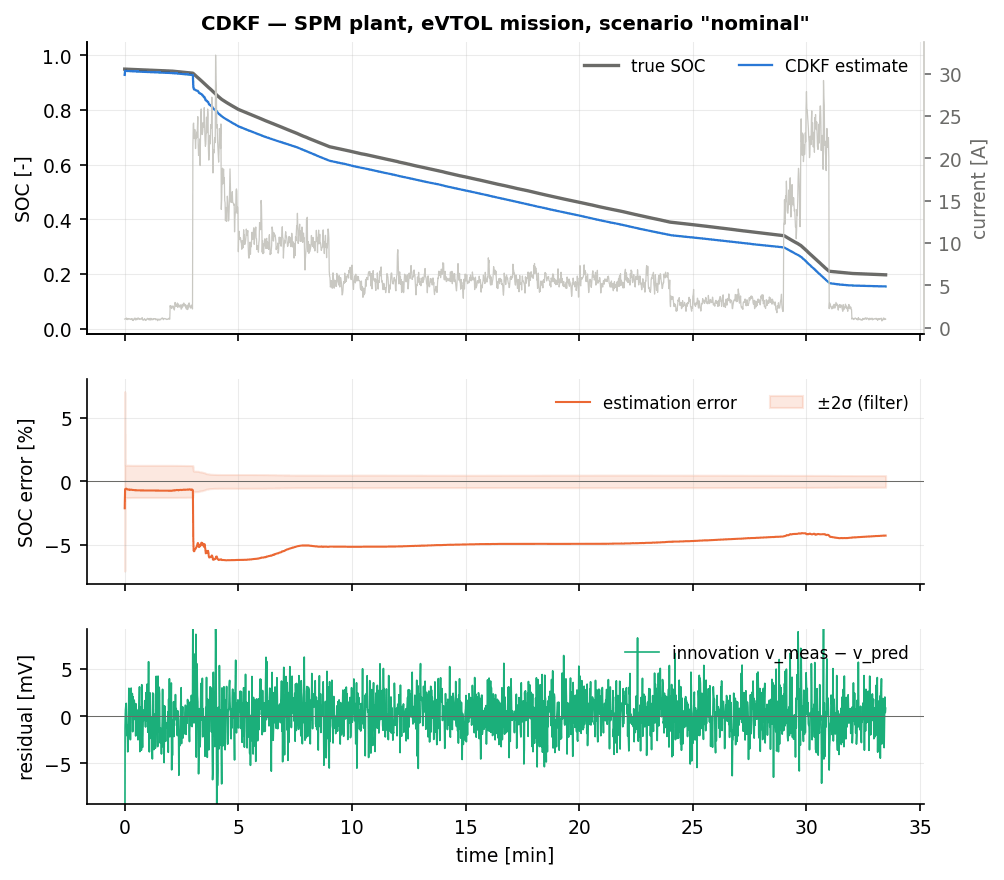
\includegraphics[width=\textwidth]{figures/cellspm_CDKF_nominal.png}
\caption{CDKF on the nominal mission with the electrochemical (SPM) plant.}
\end{figure}
The SPM block of the table is a different kind of test. The plant is the electrochemical
single-particle model; the estimator still runs a 2-RC equivalent circuit, fitted to that plant,
which leaves a \emph{structured} residual of about $4$\,mV (Butler--Volmer kinetics and
solid-phase diffusion that no 2-RC circuit can reproduce) and a slow second branch,
$\tau_2 = 556$\,s. Over a $33$-minute mission a $556$\,s pole barely relaxes, so $v_2(t)$ is
close to an affine ramp --- and so is $\ocv(\soc(t))$ while the cell discharges at a roughly
constant rate. The two channels through which the measurement sees the state,
$(\partial\ocv/\partial\soc)\,\delta\soc$ and $-\delta v_2$, are therefore nearly collinear in
the information accumulated over the flight: the pair $(\soc, v_2)$ is close to unobservable,
and no filter can decide whether a persistent few-millivolt residual belongs to the slow RC
branch or to the state of charge. Because that direction is weakly observable, a $4$\,mV
structured error maps onto \emph{several per cent} of SOC instead of the
$4\,\text{mV}/0.8\,\text{V}\approx0.5\,\%$ a well-conditioned channel would give. This
$(\soc,v_2)$ ambiguity, not the size of the residual, is the mechanism behind the
$3.7$--$4.6\,\%$ band in which the whole classical family sits.

The fifth-degree rules sit at the bad end of the band: $4.61\,\%$ on SPM \texttt{nominal}
against the EKF's $3.73\,\%$ and the LKF's $1.72\,\%$, $8.74\,\%$ on \texttt{cold} against
$7.35\,\%$, $8.24\,\%$ on \texttt{sensor\_dropout} against $5.31\,\%$, $4.90\,\%$ on
\texttt{param\_mismatch} against $3.13\,\%$. They are statistically indistinguishable from the
third-degree CKF ($4.62$, $8.72$, $8.24$, $4.81\,\%$) --- the extra degree of exactness buys
nothing at all here --- and the ordering across the family is monotone in the point spread:
LKF (frozen tangent) $1.72$, EKF/IEKF (tangent at the mean) $3.66$--$3.73$, UKF
($0.2\sigma$ points) $3.96$, the degree-three and degree-five rules ($2\sigma$ and
$2.45\sigma$) $4.61$--$4.62$. The reason is the ambiguity above: a statistical linearisation
over a wide prior returns the \emph{chord} of the OCV curve, which is steeper than the tangent
over most of the mission, so these filters believe the OCV channel is more informative than it
is and commit harder to the direction that carries the structured error. The exception is
\texttt{outliers} ($2.27\,\%$), better than on the ECM plant for everyone because the corrupted
samples widen the effective innovation covariance. Nothing diverges; every SPM error is a bias,
not a drift ($t_{\text{conv}} = 0$ throughout).

One point is specific to the divided-difference construction. On the ECM plant its second
difference is self-scaling: at $\sigma_\soc\approx10^{-3}$ the stencil shrinks below the OCV
table spacing and the $\mD^{(2)}$ term correctly vanishes, so the filter degenerates to an EKF
exactly when the EKF is right. On the SPM plant $\sigma_\soc$ stays large --- the filter is
never confident, because the residual keeps re-inflating it --- so the stencil stays wide and
the chord effect is permanently active. Self-scaling is a virtue when the covariance is
trustworthy and a liability when a structural residual keeps it open.

\section{Summary}
The DD2/CDKF is the best accuracy-per-flop sigma-point filter in this family: $9$ model
evaluations per stage buy fifth-degree moment accuracy, identical to a $33$-point cubature rule
or an $81$-point quadrature grid, and its second-difference term scales itself with $\mP$ so
that it disappears when the prior is tight. Use it as the default derivative-free filter,
particularly when analytic Jacobians are unavailable or when the measurement function is a
table. Its one parameter, $h$, should be left at $\sqrt3$ unless the function has a feature
narrower than $\sqrt3\sigma$; and like every wide-stencil method it converges slowly from a very
wide prior and is at the bad end of the family under structured model error, where an EKF or an
IEKF step is preferable.
